\documentclass[14pt]{extarticle}
% \documentclass[14pt]{article}

% \usepackage[style=authoryear,maxbibnames=9,maxcitenames=2,uniquelist=false,backend=biber,doi=false,url=false]{biblatex}
% \addbibresource{$BIB} % bibtex location
% \renewcommand*{\nameyeardelim}{\addcomma\space} % have comma in parencite
\usepackage{natbib}

\usepackage{xcolor}
\usepackage{amsmath}
\newcommand{\tuple}[1]{ \langle #1 \rangle }
%\usepackage{automata}
\usepackage{times}
\usepackage{ltablex}
\usepackage{tasks}

%%%%%% Template
\usepackage{hyperref}
\hypersetup{colorlinks=true,allcolors=blue}

\usepackage{vmargin}
\setpapersize{USletter}
\setmarginsrb{1.0in}{1.0in}{1.0in}{0.6in}{0pt}{0pt}{0pt}{0.4in}

% HOW TO USE THE ABOVE:
%\setmarginsrb{leftmargin}{topmargin}{rightmargin}{bottommargin}{headheight}{headsep}{footheight}{footskip}
%\raggedbottom
% paragraphs indent & skip:
\parindent  0.3cm
\parskip    -0.01cm

\usepackage{tikz}
\usetikzlibrary{backgrounds}

% hyphenation:
% \hyphenpenalty=10000 % no hyphen
% \exhyphenpenalty=10000 % no hyphen
\sloppy

% notes-style paragraph spacing and indentation:
\usepackage{parskip}
\setlength{\parindent}{0cm}

% let derivations break across pages
\allowdisplaybreaks

\newcommand{\orange}[1]{\textcolor{orange}{#1}}
\newcommand{\blue}[1]{\textcolor{blue}{#1}}
\newcommand{\red}[1]{\textcolor{red}{#1}}
\newcommand{\freq}[1]{{\bf \sf F}(#1)}
\newcommand{\datafreq}[2]{{{\bf \sf F}_{#1}(#2)}}

\def\qqquad{\quad\qquad}
\def\qqqquad{\qquad\qquad}

%%%%%%%%%%%%%%%%%%%%%%%%%%%%%%%%%%%%%%%%%%%%%%%%%%%%%%%%%%%%%%%%%%%%%%%%%%%%%%%%
%%%%%%%%%%%%%%%%%%%%%%%%%%%%%%%%%%%%%%%%%%%%%%%%%%%%%%%%%%%%%%%%%%%%%%%%%%%%%%%%

% fill-in-blank question style, found in https://tex.stackexchange.com/a/505089

\usepackage{ifthen}
\usepackage{tocloft}
\usepackage{exercise}
% \usepackage{xcolor}

% Set the Show Answers Boolean
\newboolean{showAns}
\setboolean{showAns}{false}
\newcommand{\showAns}{\setboolean{showAns}{true}}

% The length of the Answer line
\newlength{\answerlength}
\newcommand{\anslen}[1]{\settowidth{\answerlength}{#1}}

% ans command that indicates space for an answer or shows the answer in red
\newcommand{\ans}[1]{\settowidth{\answerlength}{\hspace{2ex}#1\hspace{2ex}}%
    \ifthenelse{\boolean{showAns}}%
        {\textcolor{red}{\underline{\hspace{2ex}#1\hspace{2ex}}}}%
        {\underline{\hspace{\answerlength}}}}%

\newcommand{\details}[1]{\settowidth{\answerlength}{#1}%
    \ifthenelse{\boolean{showAns}}%
        {\\ \textcolor{blue}{#1}}%
        {}}%

% Formatting how multiple choices Questions are formated.
\settasks{label=(\Alph*), label-width=30pt}


% Some commands for the Exercise Question package
\renewcommand{\QuestionNB}{\Large\protect\textcircled{\small\bfseries\arabic{Question}}\ }
\renewcommand{\ExerciseHeader}{} %no header
\renewcommand{\QuestionBefore}{3ex} %Space above each Q
\setlength{\QuestionIndent}{8pt} % Indent after Q number


% To create the list of answers with tocloft...
\newcommand{\listanswername}{Answers}
\newlistof[Question]{answer}{Answers}{\listanswername}

% Creates a TOC for Answers
\newcounter{prevQ}
\newcommand{\answer}[1]{\refstepcounter{answer}%
\ans{#1}%
\ifnum\theQuestion=\theprevQ%
        \addcontentsline{Answers}{answer}{\protect\numberline{}#1}% don't include the Q number
        \else%
        \addcontentsline{Answers}{answer}{\protect\numberline{\theQuestion}#1}%
        \setcounter{prevQ}{\value{Question}}%
        \fi%
        }%

% \hyphenpenalty=10000 % no hyphen
% \exhyphenpenalty=10000 % no hyphen
\sloppy              % hyphen

\newcommand{\HRule}{\rule{\linewidth}{0.5mm}}
\newcommand{\Hrule}{\rule{\linewidth}{0.3mm}}

%tocloft formatting listofanswers
\renewcommand{\cftAnswerstitlefont}{\bfseries\large}
\renewcommand{\cftanswerdotsep}{\cftnodots}
\cftpagenumbersoff{answer}
\addtolength{\cftanswernumwidth}{10pt}

\makeatletter% since there's an at-sign (@) in the command name
\renewcommand{\@maketitle}{%
  \parindent=0pt% don't indent paragraphs in the title block
  \centering
  {\Large \bfseries\textsc{\@title}} \\
  \vspace{5pt}
  {\large \textit{\@author}} \\
  \HRule \\
  \vspace{1em}
}
\makeatother% resets the meaning of the at-sign (@)


\title{ECON 2002.01 Problem Set 5 }
\author{Unit 9 \\
  \vspace{5pt}
    Hui-Jun Chen}


%%%%%%%%%%%%%%%%%%%%%%%%%%%%%%%%%%%%%%%%%%%%%%%%%%%%%%%%%%%%%%%%%%%%%%%%%%%%%%%%
%%%%%%%%%%%%%%%%%%%%%%%%%%%%%%%%%%%%%%%%%%%%%%%%%%%%%%%%%%%%%%%%%%%%%%%%%%%%%%%%
\begin{document}

\maketitle

\showAns
\listofanswer

\begin{Exercise}

\Question (OUP-U9-Q3)
The figure shows the wage-setting curve and the real wage w*. Which of the following statements is correct?
    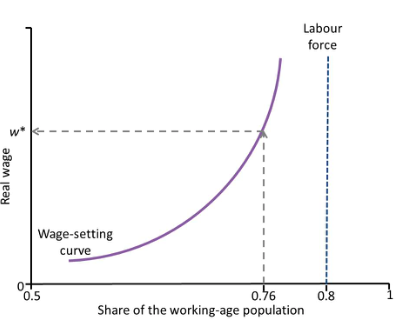
\includegraphics[width=\textwidth]{../QuestionBankImage/OUP-U9-Q3-01.png}
\answer{A}
\begin{tasks}(1)
    \task The unemployment rate is 5\%.
        \details{Unemployment rate = Unemployed / Labour force = (0.8 – 0.76)/0.8 = 5\%.}
    \task The participation rate is 76\%.
        \details{Participation rate = Labour force / Population of working age = 0.8 or 80\%.}
    \task The employment rate is 95\%.
        \details{Employment rate = Employed / Population of working age = 0.76 or 76\%.}
    \task 4\% of the population is unemployed.
        \details{Here we do not know the size of the population. However the population is bigger than the working-age population, and therefore the proportion of the population unemployed is less than 4\%.}
\end{tasks}



\Question (OUP-U9-Q14)
\answer{D}
The following diagram depicts a firm’s demand curve given the economy-wide demand, and its tangent isoprofit curve. The firm faces a linear demand curve. The workers’ average product of labour $ \lambda $ equals 1. At B, which of the following statements is correct?
    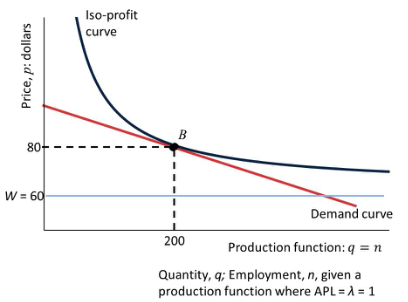
\includegraphics[width=\textwidth]{../QuestionBankImage/OUP-U9-Q14-01.png}

\begin{tasks}(1)
    \task The slope of the isoprofit curve is $-0.4$.
        \details{The slope of the isoprofit curve at B is $-(p-W)/q = -(80-60)/200 = -0.1$.}
    \task The markup is 0.1.
        \details{The markup when $\lambda = 1$ is $(p-W)/p = (80-60)/80 = 0.25$.}
    \task Profits are \$16,000.
        \details{The profit at B is $(p - W) \times  q = (80 – 60) \times  200 = \$4,000$.}
    \task The marginal rate of substitution is $-0.1$.
        \details{The MRS is the slope of the isoprofit curve, which is $-(p-W)/q = -(80-60)/200 = -0.1$.}
\end{tasks}



\Question (OUP-U9-Q23)
Which of the following statements regarding labour unions and wage bargaining is correct?
\answer{C}
\begin{tasks}(1)
    \task
The bargaining curve can be above or below the wage-setting curve.
        \details{The unions would not ask for a wage lower than the firms’ profit-maximising level. Therefore the bargaining curve is always above the wage-setting curve.}
    \task
A labour union can set both the wage level and the employment level.
        \details{The unions cannot determine how many people the firm hires.}
    \task
Unions may choose to restrain their use of bargaining power.
        \details{Demanding too high a wage may squeeze profits sufficiently, leading the firm to close down or cut back on employment. Therefore unions may choose to restrain their bargaining power.}
    \task
The unions’ bargaining power comes from their ability to shut down firms.
        \details{Shutting down firms does not help the workers. The unions’ bargaining power comes from their threat to “dismiss” the employer (at least temporarily) by going on strike i.e. withdrawing the employees’ labour from the firm.}
\end{tasks}



\Question (TEA-U9-Q2)
Which of the following statements about the wage-setting curve is correct?
\answer{B}
\begin{tasks}(1)
    \task
The wage-setting curve depicts the workers’ reservation wage for different levels of economy-wide employment.
        \details{The wage-setting curve depicts the real wage necessary to provide workers with incentives to work hard (which is higher than their reservation wage), for different levels of economy-wide employment.}
    \task
At each point (U, w) on the wage-setting curve, the workers are choosing their best response effort level given the real wage (w) and unemployment rate (U).
        \details{This is true. Each point (U, w) on the wage-setting curve is derived as the point of tangency between the workers’ best response function (their best choice of effort per hour for each w, given U) and the employers’ isocost line.}
    \task
A lower unemployment rate shifts the wage-setting curve to the left.
        \details{A lower unemployment rate shifts the workers’ best response function for effort exerted given the wage level to the right. This means that the employers need to offer a higher wage to induce a higher effort level. This is a movement up along the wage-setting curve and not a shift of the entire curve, since employment is endogenous (the horizontal axis variable).}
    \task
An exodus of European workers due to Brexit would, ceteris paribus, result in a downward shift of the UK’s wage-setting curve.
        \details{With the balance of job seekers and vacancies shifting in favour of the remaining workers, their best response function shifts to the right, resulting in the wage-setting curve shifting up.}
\end{tasks}


\Question (TEA-U9-Q3)
Which of the following statements about the price-setting curve is correct?
\answer{C}
\begin{tasks}(1)
    \task
The price-setting curve depicts the firms’ profit-maximising price level for different levels of economy-wide employment.
        \details{The price-setting curve depicts the real wage paid when firms choose their profit-maximising price, for different levels of economy-wide employment.}
    \task
Firms have to pay a higher real wage when the employment rate is higher. Therefore the price-setting curve is upward-sloping.
        \details{The price-setting curve represents the level of the real wage consistent with the firms’ profit-maximising markup over costs. It is independent of the level of employment in the economy, and therefore it is a horizontal line.}
    \task
At points below the price-setting curve, the firms are setting prices too high compared to their profit-maximising level.
        \details{The price-setting curve represents the profit-maximising real wage. At points below the curve the real wage is lower than the level consistent with the firm’s profit-maximising markup, and therefore the markup, and hence the price, is too high.}
    \task
The reduction in competition from Europe due to Brexit would result in the UK’s price-setting curve shifting up.
        \details{Lower competition means a higher markup. With the workers’ APL unaffected this leads to a fall in the real wage. Therefore the price-setting curve shifts down.}
\end{tasks}



\Question (ECO-U9-Q1)
Which of the following statements is correct?
\answer{D}
\begin{tasks}(1)
    \task
To maximize profits, firms set the wage at the level where the workers are indifferent between working and not working.
        \details{In order to motivate employees to work hard and well, firms set the wage sufficiently high so that workers receive an employment rent, in other words, there is a nonzero cost of job loss.}
    \task
Firms aim to set as high a price as possible.
        \details{There is a trade-off between a higher price/markup and quantity of sales. A firm chooses the price at which its profit is maximized.}
    \task
In equilibrium, the wage clears the labour market, so there is no unemployment.
        \details{In labour market equilibrium there is involuntary unemployment, as the wage has to be set at a level higher than the full-employment level in order to motivate employees to work hard and well.}
    \task
If all firms set the same price and pay the same nominal wage, then the higher the real wage that they pay, the lower is their markup.
        \details{The real wage is W/P while the markup is $(P - W)/P = 1 - (W/P)$. So the higher the former, the lower the latter.}
\end{tasks}



\Question (UCL-J17-Q14)
In the equilibrium of the labour market:
\answer{B}
\begin{tasks}(1)
    \task
There is excess demand for workers to make sure the workers put in sufficient effort.
        \details{There is excess supply of labour (involuntary unemployment) to make sure the workers put in sufficient effort.}
    \task
The greater the level of labour productivity, the higher the real wage.
        \details{Workers are paid according to their productivity, so higher productivity levels correspond to higher wages.}
    \task
The price-setting curve lies above the average product of labour.
        \details{The price-setting curve lies below the average product of labour.}
    % \task
    %     \details{}
\end{tasks}



\Question (OUP-U9-Q22)
The figure describes the effect of immigration on unemployment in the labour market. The labour market equilibrium is at A and C before and after the influx of immigration, respectively. Based on this figure, which of the following statements is correct?
    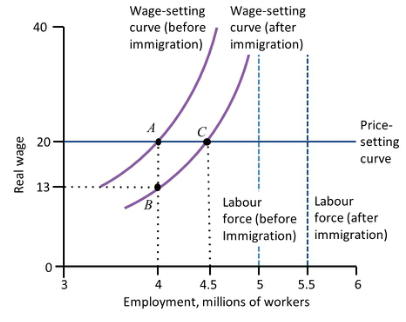
\includegraphics[width=\textwidth]{../QuestionBankImage/OUP-U9-Q22-01.png}

\answer{B}
\begin{tasks}(1)
    \task
All incumbent workers are unaffected while the labour market adjusts.
        \details{Workers face a temporary real wage cut from \$20 to \$13.}
    \task All incumbent workers are no worse off in the new equilibrium.
        \details{This is true as their employment status is unaffected and the real wage returns to \$20.}
    \task The unemployment rate is unchanged in the new equilibrium.
        \details{The number of unemployed is unchanged at 1 million before and after immigration. However the size of the labour force increases, so the unemployment rate drops after the immigration.}
    \task Firms claim a higher markup in the new equilibrium.
        \details{The average product of labour and the real wage are unchanged in the new equilibrium. Therefore the markup is also unchanged.	}
\end{tasks}



\Question (OUP-U9-Q1)
Consider an economy with firms selling differentiated products, where the only input to production is labour. Which of the following statements is correct?
\answer{D}
\begin{tasks}(1)
    \task Firms make no economic rent.
        \details{With differentiated products, firms make profits above normal profits.}
    \task Workers receive no employment rent.
        \details{A positive economic rent is required in order to induce workers to exert effort.}
    \task Firms choose the level of nominal wage that corresponds to the workers’ maximum effort.
        \details{Firms choose the lowest nominal wage they can pay without undermining the workers’ motivation to work. It may not be optimal for firms to choose a high wage even if it increases worker effort, because costs may increase more than revenues (hence profits may fall).}
    \task
	The more inelastic the demand curve faced by the firm, the higher the markup set by the firm.
        \details{Inelastic demand means a steeper demand curve, so the firm has more market power. Therefore it is able to set a higher markup.}
\end{tasks}


\Question (OUP-U9-Q17)
The figure depicts the labour market when there has been a negative aggregate demand shock. Which of the following statements is correct?
\answer{A}
    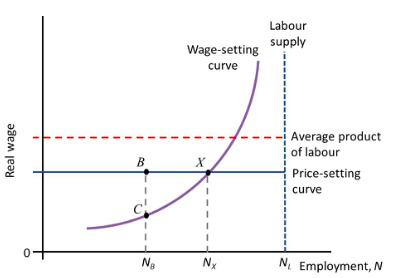
\includegraphics[width=\textwidth]{../QuestionBankImage/OUP-U9-Q17-01.png}
\begin{tasks}(1)
    \task B is not a Nash equilibrium outcome.
        \details{B is above the wage-setting curve. This means that the firms are able to increase profits by reducing their wage offer, without incurring a loss in the effort exerted by the workers. Therefore, given workers' behaviour, firms are not choosing their optimal response at B i.e. B is not a Nash equilibrium.}
    \task C is a Nash equilibrium outcome.
        \details{C is below the price-setting curve. This means that the firms are able to increase profits by restoring their profit-maximising markup away from C. Therefore it is not a Nash equilibrium.}
    \task At C, firms are able to make higher profits by increasing the price.
        \details{At C, the real wage is too low. Therefore the firms would reduce their price to re-attain their profit-maximising markup.}
    \task Moving from B to C eliminates cyclical unemployment.
        \details{Cyclical unemployment is $N_X - N_B$, which is not eliminated by moving from B to C}
\end{tasks}

\end{Exercise}

\end{document}
